\فصل{مفاهیم و معماری‌های مرتبط}
\قسمت{مقدمه}

\پاراگراف{}
راه‌اندازی و استقرار سرویس در صنعت مخابرات به طور سنتی بر این اساس است که اپراتورهای شبکه، سخت‌افزارهای و نرم‌افزارهای مناسب هر کارکرد در سرویس را در زیرساخت خود مستقر کنند.
فراهم کردن نیازمندی‌هایی مانند پایداری و کیفیت سرویس بالا منجر به اتکای فراهم کنندگان سرویس بر تجهیزات اختصاصی می‌شود.
نیازمندی کاربران به سرویس‌های متنوع و عموما با عمرکوتاه و نرخ بالای ترافیک نیز افزایش یافته است.
بنابراین فراهم کنندگان سرویس‌ها باید مرتبا و به صورت پیوسته تجهیزات فیزیکی جدید را خریده، انبارداری کرده و مستقر کنند که باعث افزایش هزینه‌های فراهم کنندگان سرویس می شود[1].
از سوی دیگر در تحقیقاتی که اخیرا انجام شده است، نشان داده شده که تعداد سخت افزارهای خاص منظوره نصب شده برای کارکردهای شبکه قابل مقایسه با تعداد سوییچ ها و مسیریاب‌های شبکه
است[4].
با افزایش تعداد تجهیزات، پیدا کردن فضای فیزیکی برای استقرار تجهیزات جدید به مرور دشوارتر می‌شود.
علاوه بر این باید افزایش هزینه و تاخیر ناشی از آموزش کارکنان برای کار با تجهیزات جدید را نیز در نظر گرفت.
همچنین اغلب کارایی و قابلیت‌های سخت افزارها و نرم افزارهای خاص منظوره که از سمت فروشندگان تجهیزات ارائه می‌شود محدود به انتخاب‌های فروشندگان است
و خریداران تجهیزات قادر به سفارشی‌سازی تجهیزات خریداری شده نیستند.
بدتر این ‍که هر چه نوآوری سرویس‌ها و فناوری شتاب بیشتری می‍گیرد، چرخه عمر سخت‌افزارها کوتاه‍تر می‍شود که مانع از ایجاد نوآوری در سرویس‌های شبکه می‌شود[2].

\پاراگراف{}
در روش سنتی استقرار سرویس شبکه، ترافیک کاربر باید از تعدادی کارکرد شبکه به ترتیب معینی عبور کند تا یک مسیر پردازش ترافیک ایجاد شود.
در حال حاضر این کارکردها به صورت سخت افزاری به یکدیگر متصل هستند و ترافیک با استفاده از جداول مسیریابی به سمت آن ها هدایت می‌شود.
چالش اصلی این روش در این است که استقرار و تغییر ترتیب کارکردها دشوار است.
به عنوان مثال، به مرور زمان با تغییر شرایط شبکه نیازمند تغییر همبندی و یا مکان کارکردها برای سرویس‌دهی بهتر به کاربران هستیم
که نیاز به جا به جایی کارکردها و تغییر جداول مسیریابی دارد.
در روش سنتی این کار سخت و هزینه‌بر است که ممکن است خطاهای بسیاری در آن رخ دهد.
از جنبه دیگر، تغییر سریع سرویس‌های مورد نظر کاربران نیازمند تغییر سریع در ترتیب کارکردها است که در روش فعلی این تغییرات به سختی صورت گیرد.
بنابراین اپراتورهای شبکه نیاز به شبکه‌های قابل برنامه ریزی و ایجاد زنجیره سرویس کارکردها به صورت پویا پیدا کرده‌اند[3]، [4].‍‍

\پاراگراف{}
دو فناوری برای پاسخ گویی به این چالش ها مطرح شد: مجازی‌سازی کارکرد شبکه \متن‌لاتین{(NFV)} و زنجیره‌سازی کارکردهای سرویس \متن‌لاتین{(SFC)}.‍
هدف از مجازی‌سازی کارکردهای شبکه این است که کارکردها بتوانند بر روی سخت افزارهای استاندارد اجرا شوند تا
نیاز به تجهیزات سخت‌افزاری خاص منظوره کاهش یابد.
از طرف دیگر زنجیره‌سازی کارکردهای سرویس امکان تعریف زنجیره کارکردها به صورت پویا و در هر زمان را ارائه می‌کند که تغییر در زیرساخت فیزیکی را کاهش می‌دهد.

\پاراگراف{}
از آنجایی که از مفاهیم این فناوری ها برای طراحی و تعریف مسئله در این رساله استفاده شده است، نیازمند آشنایی با مفاهیم ابتدایی و اصول اولیه آن ها خواهیم بود. بنابراین در این فصل به صورت خلاصه اجزای این فناوری ها را مرور خواهیم کرد و کاربردها، چالش ها و مسائل تحقیقاتی که در هر یک از این معماری ها وجود دارد را مورد بررسی قرار خواهیم داد.

\قسمت{مجازی‌سازی کارکرد شبکه}
\پاراگراف{}
مجازی‌سازی کارکرد شبکه اصل جداسازی کارکرد شبکه به وسیله انتزاع سخت‌افزاری مجازی از سخت‌افزاری است که بر روی آن اجرا می‌شود.
هدف مجازی‌سازی کارکرد شبکه تغییر روش اپراتورهای شبکه در طراحی شبکه با تکامل مجازی‌سازی استاندارد فناوری اطلاعات به منظور تجمیع تجهیزات شبکه در سرورهای استاندارد،
سوییچ‌ها و ذخیره‌سازها با توان بالا است.
یک سرور استاندارد با توان بالا سروری است که توسط اجزای استاندارد شده فناوری اطلاعات، مانند معماری \متن‌لاتین{x86}، ساخته‌شده و در تعداد بالایی، مانند میلیون، فروخته می‌شود.
ویژگی اصلی این سرورها این است که اجزای آن‌ها به راحتی از فروشندگان مختلف قابل خریداری و تعویض است.
این تجهیزات می‌توانند در مراکز داده، گره‌های شبکه، یا مکان کاربران انتهایی قرار بگیرند.
این روند در \رجوع{fig:nfv-opinion} نیز توصیف شده است. با استفاده از مجازی‌سازی کارکرد شبکه، انواع کارکردهای شبکه مانند دیواره آتش و \متن‌لاتین{NAT} را می‌توان
به صورت یک برنامه نرم‌افزاری از فروشندگان مختلف تهیه کرد و آن‌ها را بر روی سرورهای با توان بالا اجرا کرد که نیاز به نصب تجهیزات خاص منظوره و جدید را برطرف می‌سازد[2].

\پاراگراف{}
مزایا و اهداف اساسی که \متن‌لاتین{NFV} برای تحقق و دست‍یابی به آن‍ها شکل گرفته است عبارتند از[6]:

\شروع{فقرات}
\فقره کاهش هزینه‌های تجهیزات و مصرف انرژی از طریق تجمیع کارکردها بر روی سرورها و در نتیجه کاهش تعداد تجهیزات
\فقره کاهش نیاز به آموزش کارکنان، افزایش دسترسی‌پذیری به سخت‌افزار و کاهش زمان بازیابی از خرابی سخت‌افزار به علت استفاده از سخت‌افزارهای استاندارد و عمومی
\فقره افزایش سرعت عرضه محصول به بازار با کوتاه کردن چرخه نوآوری و تولید. در واقع مجازی‌سازی کارکرد شبکه به اپراتورهای شبکه کمک می‌کند تا چرخه بلوغ محصول را به اندازه قابل توجهی کاهش دهند.
\فقره امکان‍پذیر بودن تعریف سرویس مورد نظر بر اساس نوع مشتری یا محل جغرافیایی. مقیاس سرویس‌ها می‍تواند به سرعت، بر اساس نیاز، گسترش یا کاهش یابد.
\فقره تشویق به ایجاد نوآوری و ارائه سرویس‌های جدید و دریافت جریان‌های درآمدی تازه با سرعت بالا و ریسک پایین.
\فقره افزایش توانایی مقابله با خرابی کارکردها، قابلیت به اشتراک گذاری منابع بین کارکردها و پشتیابی از چند مشتری
\پایان{فقرات}

\پاراگراف{}
سازمان‌های استانداردگذاری متعددی در استانداردسازی فناوری مجازی‌سازی کارکرد شبکه دخیل هستند که شاخص‌ترین آن‌ها موسسه استانداردهای مخابراتی اروپا\پانویس{European Telecommunications Standards Institute} \متن‌لاتین{(ETSI)} است.
در اواخر سال ۲۰۱۲ \متن‌لاتین{ETSI NFV ISG} توسط هفت اپراتور جهانی شبکه به منظور ارتقا ایده مجازی‌سازی کارکرد شبکه تأسیس شد.
\متن‌لاتین{NFV ISG} تبدیل به یک بستر صنعتی اصلی برای توسعه چارچوب معماری \متن‌لاتین{NFV} و نیازمندی‌های آن شده است
و اکنون بیش از ۲۵۰ سازمان با آن همکاری می‌کنند. اسناد معماری \متن‌لاتین{NFV} به صورت عمومی و رایگان توسط \متن‌لاتین{ETSI NFV ISG} منتشر می‌شود.
ما در این رساله برای توصیف معماری \متن‌لاتین{NFV} از اسناد ارائه شده این سازمان استفاده می‌کنیم.

\زیرقسمت{اجزای معماری \متن‌لاتین{NFV}}

\پاراگراف{}
در این بخش مؤلفه‌های تشکیل‌دهنده معماری \متن‌لاتین{NFV} شرح داده می‌شوند.
هر یک از اجزای معماری می‌توانند توسط تولیدکنندگان متفاوتی تأمین شوند و به وسیله واسط‌هایی که توسط معماری \متن‌لاتین{NFV} توصیف شده‌اند
با یکدیگر در ارتباط باشند.
بنابراین معماری \متن‌لاتین{NFV} توصیف شده توسط \متن‌لاتین{ETSI} راه‌حلی با قابلیت مشارکت و هماهنگی چندین تولیدکننده مختلف را دارد.
مؤلفه‌های اصلی چارچوب معماری \متن‌لاتین{NFV} که در \رجوع{fig:nfv-architecture} دیده می‌شوند عبارتند از:

\شروع{فقرات}
\فقره \متن‌لاتین{NFVI}\\ شامل منابع سخت افزاری و نرم افزاری لازم برای اجرای \متن‌لاتین{VNF}ها
\فقره \متن‌لاتین{Service}\\ شامل \متن‌لاتین{VNF}ها که کارکردهای شبکه را پیاده‌سازی کرده‌اند، \متن‌لاتین{EMS} برای مدیریت \متن‌لاتین{VNF}ها و \متن‌لاتین{OSS/BSS} برای ارتباط با سیستم‌های مدیریت سنتی
\فقره \متن‌لاتین{MANO}\\ که وظیفه مدیریت و هماهنگی سرویس ها و تخصیص منابع را برعهده دارد و از سه بخش
\متن‌لاتین{NFVO}
، \متن‌لاتین{VIM}
و \متن‌لاتین{VNFM}
تشکیل شده است.
\پایان{فقرات}
در ادامه به توصیف اجزای ذکر شده از اسناد \متن‌لاتین{ETSI} می پردازیم[6]، [7]، [8] و [9].

\زیرزیرقسمت{\متن‌لاتین{NVFI}}
\پاراگراف{}
مولفه \متن‌لاتین{NFVI} شامل تمام نرم‌افزارها، مانند \متن‌لاتین{Hypervisor}، و سخت‌افزارهایی است که با همکاری یکدیگر منابع زیرساخت برای استقرار \متن‌لاتین{VNF}ها را فراهم می‌کنند.
سخت‌افزارهای موجود در زیرساخت \متن‌لاتین{NFV} به سه دسته منابع پردازشی، منابع ذخیره سازی و شبکه ارتباطی دسته بندی می شوند.
\متن‌لاتین{Hypervisor} یک لایه نرم‌افزاری است که سخت‌افزارهای زیرساخت را مجازی کرده و انتزاعی از آن‍ها به دست می‌دهد.

\پاراگراف{}
این مولفه می‌تواند شامل کارکردهای شبکه به صورت کامل مجازی نشده نیز باشد.
در این مولفه هر جایی که یک کارکرد شبکه به صورت یک \متن‌لاتین{VNF} می تواند استقرار یابد یک \متن‌لاتین{NFVI-PoP} نامیده می‌شود.
به عنوان مثال یک سرور مجازی شده و یا یک مرکز داده مجازی شده را می توان به عنوان \متن‌لاتین{NFVI-PoP} در نظر گرفت.

\زیرزیرقسمت{\متن‌لاتین{VNF}}

\پاراگراف{}
یک \متن‌لاتین{VNF} پیاده‌سازی از یک کارکرد شبکه است که می‌تواند بر روی \متن‌لاتین{NFVI} استقرار یابد.
یک نمونه\پانویس{instance} از \متن‌لاتین{VNF}، نتیجه ایجاد نمونه در زمان اجرا از برنامه \متن‌لاتین{VNF} و مولفه‌های آن با رعایت نیازمندی‌های توصیف شده لازم است.
در حقیقت یک نمونه را می‌توان با استفاده از اجرای برنامه یا تصویر\پانویس{image} \متن‌لاتین{VNF} در یک ماشین مجازی و اختصاص منابع محاسباتی، پردازشی و شبکه به آن ایجاد کرد.
هر \متن‌لاتین{VNF} می‌تواند از یک یا چند مولفه \متن‌لاتین{(VNFC)} تشکیل شود که هر یک از این مولفه‌ها خود می‌توانند در یک ماشین مجازی اجرا شوند.
برای ایجاد نمونه از یک \متن‌لاتین{VNF}، از همه \متن‌لاتین{VNFC}های آن باید نمونه ایجاد شود.
به عنوان یک مثال از \متن‌لاتین{VNF} می‌توان کارکرد دیواره آتش مجازی شرکت \متن‌لاتین{CISCO} به نام \متن‌لاتین{ASAv} را نام برد که مشخصات آن در شکل 3 نمایش داده شده است.
همانگونه که در این شکل مشاهده می‌شود، چهار قالب مختلف \متن‌لاتین{ASAv} تعریف شده که هر کدام نیازمندی های منابع پردازشی، حافظه و ذخیره سازی متفاوتی دارند و متناسب با منابع اختصاص یافته به آن‌ها،
توانایی پردازش ترافیک مشخصی را می‌توانند ارائه کنند که با عنوان \متن‌لاتین{Throughput} در شکل مشخص شده است. برای استقرار هر یک از این قالب‌ها باید یک ماشین مجازی مطابق با
مشخصات نمایش داده شده در این شکل آماده شود و تصویر \متن‌لاتین{ASAv} به آن داده شود.
البته این روند برای \متن‌لاتین{ASAv} به صورت خودکار و با استفاده از یک قالب استقرار که همراه با \متن‌لاتین{VNF} دانلود می‌شود انجام می‌شود.
هر یک از این قالب‌ها نیاز به مجوزهای متفاوت دارند و هزینه‌های استفاده از آن‌ها متفاوت است.

\پاراگراف{}
هر \متن‌لاتین{VNF} توسط توصیف‌گر\پانویس{descriptor} \متن‌لاتین{VNF(VNFD)} توصیف می‌شود که شامل توصیف \متن‌لاتین{VNF} و
نیازمندی‌های لازم برای استقرار و همچنین رفتار \متن‌لاتین{VNF} در زمان اجرا است.
دو نوع مقیاس پذیری برای نمونه‌های یک \متن‌لاتین{VNF} در زمان اجرا تعریف می‌شود. مقیاس پذیری افقی و عمودی. در اسناد \متن‌لاتین{ETSI} این مقیاس پذیری‌ها برای \متن‌لاتین{VNFC}ها به صورت زیر تعریف شده است:

\شروع{فقرات}

\فقره افزایش مقیاس افقی\\ نمونه‌های جدیدی از \متن‌لاتین{VNFC}ها ایجاد می‌شود.
\فقره افزایش مقیاس عمودی\\ منابع پردازشی، ذخیره‌سازی و یا شبکه‌ای بیشتری به نمونه‌های ایجاد شده از \متن‌لاتین{VNFC}ها داده می‌شود.
\فقره کاهش مقیاس افقی\\ نمونه‌های ایجاد شده از \متن‌لاتین{VNFC}ها خاتمه می‌یابند.
\فقره کاهش مقیاس عمودی\\ منابع داده شده به نمونه‌های \متن‌لاتین{VNFC}ها از آن‌ها گرفته می‌شود.
\پایان{فقرات}

\پاراگراف{}
البته همانگونه که در تعریف \متن‌لاتین{ETSI}، مقیاس پذیری برای \متن‌لاتین{VNFC}ها تعریف شده، می‌توان آن را برای \متن‌لاتین{VNF} نیز تعریف کرد.
افزایش یا کاهش مقیاس افقی و عمودی می‌تواند به صورت خودکار بر اساس شرایط مشخص شده در \متن‌لاتین{VNFD} انجام شود یا از طریق واسط‌های مدیریتی و بر اساس شرایط شبکه تصمیم گیری شود.
همچنین چهار روش برای توزیع بار\متن‌لاتین{Load Balancing} بین نمونه‌های مختلف یک \متن‌لاتین{VNF} به شرح زیر بیان شده است:

\شروع{فقرات}

\فقره \متن‌لاتین{VNF-Internal Load balancer}\\
در این حالت فرض می‌شود که یک \متن‌لاتین{VNFC} داخل \متن‌لاتین{VNF} وجود دارد که توزیع و جمع آوری ترافیک را انجام می‌دهد.
در این حالت نمونه‌های تکثیر شده \متن‌لاتین{VNFC} از \متن‌لاتین{VNF}های دیگر قابل مشاهده نیستند. این حالت در شکل 4 نمایش داده شده است.

\فقره \متن‌لاتین{VNF-External load balancer}\\
در این حالت یک \متن‌لاتین{VNF} به عنوان توزیع کننده بار عمل می کند و ترافیک را بین نمونه های ایجاد شده از \متن‌لاتین{VNF} توزیع می‌کند.
از دید \متن‌لاتین{VNF} های دیگر، کل مجموعه به صورت یک \متن‌لاتین{VNF} دیده می‌شود. این حالت در شکل شکل 5 نمایش داده شده است.

\فقره \متن‌لاتین{End-to-End Load balancer}\\
در این حالت نمونه‌های ساخته شده از \متن‌لاتین{VNF} به صورت \متن‌لاتین{VNF}های مجزا دیده می‌شوند.
در این حالت \متن‌لاتین{Peer NF} خود قابلیت توزیع ترافیک بین نمونه‌های ایجاد شده را دارد. مثالی از این حالت در شکل 6 نمایش داده شده است.

\فقره \متن‌لاتین{Infrastructure network load balancer}\\
در این حالت، نمونه‌های ایجاد شده از \متن‌لاتین{VNF}، به صورت یک \متن‌لاتین{VNF} واحد دیده می‌شوند
و یک توزیع کننده بار در زیرساخت (به عنوان مثال در \متن‌لاتین{Hypervisor}) وظیفه توزیع و جمع آوری ترافیک از/به نمونه‌های ایجاد شده را برعهده دارد.
مثالی از این حالت در شکل 7 نمایش داده شده است.

\پایان{فقرات}

\زیرزیرقسمت{\متن‌لاتین{EM}}

\پاراگراف{}
این مولفه کارکردهای \متن‌لاتین{FCAPS}\پانویس{Fault,Config,Accounting,Performance,Security management}
را برای \متن‌لاتین{VNF} ها انجام می‌دهد که شامل مدیریت خطا، پیکربندی، امنیت، حسابداری و کارایی برای کارکردی است که \متن‌لاتین{VNF} ارائه می‌دهد.
این مولفه ممکن است آگاه از مجازی‌سازی کارکرد باشد و با همکاری \متن‌لاتین{VNFM} عملکردهای خودش را انجام بدهد.

\زیرزیرقسمت{\متن‌لاتین{OSS/BSS}}

\پاراگراف{}
این مولفه، ترکیبی از سایر بخش های عملکردهای اپراتور است که در چارچوب معماری NFV ارائه شده از طرف ETSI قرار نمیگیرند. به عنوان مثال می تواند شامل مدیریت سیستم های Legacy باشد.

\زیرزیرقسمت{\متن‌لاتین{NFVO}}

\پاراگراف{}
این مولفه بخشی از مولفه MANO است که وظیفه تخصیص منابع به سرویس را برعهده دارد. یکی از مهم ترین اجزای سرویس گراف VNF-FG است که بیانگر VNF های سرویس و ارتباطات بین آن ها است. وظیفه اصلی مولفه NFVO ایجاد نمونه از سرویس و مدیریت چرخه حیات آن است. ایجاد نمونه از سرویس شامل ایجاد نمونه از VNF های تشکیل دهنده آن و ایجاد ارتباط بین نمونه ها است. سایر وظایف مولفه VNFO به شرح زیر است:
    • مدیریت چرخه حیات سرویس شبکه
    • مدیریت و هماهنگی منابع مورد نیاز NFVI بین چندین VIM
    • مدیریت منابع و ایجاد نمونه از VNF ها با هماهنگی VNFM
    • مدیریت منابع و نمونه سازی VNFM
    • مدیریت همبندی نمونه ساخته شده از سرویس شبکه مانند ایجاد، حذف و به روز رسانی VNF-FG
    • مدیریت قالب های استقرار سرویس شبکه و VNF ها مانند اعتبار سنجی قالب ها
همچنین این مولفه مسئولیت مشخص کردن مکان فیزیکی نمونه های ایجاد شده از VNFها را برعهده دارد.

\زیرزیرقسمت{\متن‌لاتین{NFVM}}

\پاراگراف{}
این مولفه مسئولیت مدیریت چرخه حیات نمونه های ایجاد شده ازVNF ها را برعهده دارد. بنابراین فرض می شود هر نمونه ایجاد شده از هر VNF، به یک VNFM اختصاص یافته است. مهم ترین وظایف این مولفه به شرح زیر است:
    • پیکربندی و نمونه سازی از VNF ها
    • گسترش و یا کاهش مقیاس پذیری افقی یا عمودی برای نمونه های ایجاد شده از VNFها
    • مدیریت نمونه های ایجاد شده شامل  تغییرات، به روز رسانی برنامه ها و خاتمه دادن به نمونه ها
مولفه VNFM با استفاده از VNFD، از VNF نمونه ایجاد می کند و مدیریت چرخه حیات آن را انجام می دهد. منابع پردازشی، محاسباتی و شبکه مطابق با توصیفات گفته شده در VNFD به نمونه های آن اختصاص می یابند.

\زیرزیرقسمت{‌VIM}

\پاراگراف{}
این مولفه مسئولیت مدیریت چرخه حیات نمونه‌های ایجاد شده از VNFها را برعهده دارد. بنابراین فرض می‌شود هر نمونه ایجاد شده از هر VNF، به یک VNFM اختصاص یافته است.
مهم ترین وظایف این مولفه به شرح زیر است:

\شروع{فقرات}

\فقره پیکربندی و نمونه‌سازی از VNFها
\فقره گسترش و یا کاهش مقیاس پذیری افقی یا عمودی برای نمونه های ایجاد شده از VNFها
\فقره مدیریت نمونه‌های ایجاد شده شامل تغییرات، به روزرسانی برنامه‌ها و خاتمه دادن به نمونه‌ها

\پایان{فقرات}

مولفه VNFM با استفاده از VNFD، از VNF نمونه ایجاد می‌کند و مدیریت چرخه حیات آن را انجام می‌دهد.
منابع پردازشی، محاسباتی و شبکه مطابق با توصیفات گفته شده در VNFD به نمونه‌های آن اختصاص می‌یابند.

\زیرقسمت{سرویس شبکه و اجزای آن}

\پاراگراف{}
یک سرویس شبکه را می‌توان به صورت یک گراف جلورانی\پانویس{Forwarding Graph} از کارکردهای شبکه (NF-FG) که به یکدیگر از طریق زیرساخت شبکه متصل هستند دید.
کارکردهای شبکه می‌تواند توسط یک یا چند اپراتور ارائه شده باشند. نقاط انتهایی\پانویس{Endpoint} سرویس را می‌توان به صورت گره‌های گراف و ارتباطات
میان کارکردها را توسط لینک‌های گراف مدل سازی کرد که لینک های گراف می توانند، یک طرفه یا دو طرفه، چند پخشی یا همه پخشی باشند. مثالی از یک سرویس شبکه در شکل 8 نمایش داده شده است. در این شکل، یک سرویس شبکه انتها به انتها از طریق نقاط انتهایی A و B ایجاد شده که شامل یک NF-FG داخلی است. این NF-FG خود شامل سه کارکرد شبکه است که به یکدیگر متصل هستند[6].

\پاراگراف{}
در صورتی که در یک NF-FG حداقل یکی از این کارکردها VNF باشد، به آن VNF-FG گفته می‌شود[8].
در صورتی که فرض کنیم همه NFهای شکل 8، VNF هستند می‌توان آن را مطابق شکل 9 نمایش داد. در این شکل NF 2 خود توسط سه VNF پیاده سازی شده است.

\پاراگراف{}
مشخص است که گراف VNF-FG صرفا ارتباطات بین VNFها رو مشخص می‌کند ولی ترتیب عبور ترافیک از کارکردها را بیان نمی‌کند.
ترتیب عبور ترافیک از کارکردها توسط NFP\پانویس{Network Forwarding Path} بیان می‌شود که یکی از اجزای VNF-FG است و هر VNF-FG باید حداقل یک NFP داشته باشد.

\پاراگراف{}
همانگونه که گفته شد، هدف NFV تغییر در نحوه ارائه سرویس سنتی شبکه است.
به همین دلیل در این بخش نحوه تعریف سرویس شبکه در معماری NFV و اجزای آن را بررسی می‌کنیم. این اجزا در تعریف مسائل بیان شده در این رساله مطرح می‌شوند.

\زیرزیرقسمت{توصیف سرویس در معماری NFV}

\پاراگراف{}
در معماری NFV سرویس شبکه به صورت مجموعه از کارکردهای فیزیکی، مجازی و لینک‌های مجازی تعریف می شود که توسط مشخصات کارکردی و غیرکارکردی‌اش توصیف می‌شود.
لینک‌های مجازی کارکردها را به یکدیگر و به نقاط انتهایی متصل می‌کند و مجموعه لینک‌های مجازی همبندی اتصالات شبکه\پانویس{Network Connection Topology}
(NCT) را تشکیل می‌دهند. یک سرویس شبکه توسط اجزای اطلاعاتی\پانویس{Information Element} زیر توصیف می‌گردد:

\شروع{فقرات}
\فقره اجزای اطلاعاتی توصیف کننده سرویس شبکه
\فقره اجزای اطلاعاتی توصیف کننده VNFهای سرویس
\فقره اجزای اطلاعاتی توصیف کننده لینک‌های مجازی سرویس
\فقره اجزای اطلاعاتی توصیف کننده VNF-FG
\فقره اجزای اطلاعاتی توصیف کننده PNFهای سرویس
\پایان{فقرات}

این اجزای اطلاعاتی به دو صورت در معماری NFV استفاده می‌شوند:

\شروع{شمارش}
\فقره به صورت توصیف کننده که هنگام ساختن نمونه، به عنوان قالب ایجاد نمونه به کار می‌رود.
\فقره به صورت رکوردهای حاوی اطلاعات نمونه‌های ایجاد شده که در زمان اجرا به کار می‌رود.
\پایان{شمارش}

\پاراگراف{}
بنابراین مشخصات کارکردها توسط توصیف کننده‌ها، توصیف می‌شوند و رکوردها پس از نمونه سازی ایجاد می شوند که بیانگر مشخصات نمونه های ایجاد شده و اطلاعات زمان اجرا هستند.
با این توصیف، NSR، VNFR، VLR، VNF-FGR، رکوردهای ایجاد شده متناظر با توصیف کننده های NSD، VNFD، VLD، VNF-FGD هستند. مولفه NFVO، توصیف کننده های NSD، VNF-FGD و VLD را در کاتالوگ سرویس بارگذاری می کند. توصیف کننده VNF یعنی VNFD همراه با VNF و به عنوان بخشی از بسته VNF بارگذاری می شود. چگونگی استقرار PNFD ها خارج از استاندارد ETSI است. در این بخش به صورت خلاصه اجزای سرویس را شرح می دهیم. اطلاعات تکمیلی این بخش در پیوست قرار داده شده است.

\زیرزیرقسمت{NSD}

\پاراگراف{}
هر سرویس شبکه توسط توصیف‌گر سرویس شبکه (NSD) توصیف می‌شود که اجزای تشکیل دهنده سرویس را توصیف می کند. مهمترین  اجزای NSD عبارتند از
پارامترهای نظارت و قالب‌های استقرار سرویس.
پارامترهای نظارت پارامترهایی هستند که لازم است برای سرویس، نظارت شوند.
به عنوان پارامترهای کیفیت سرویس جزئی از پارامترهای نظارت هستند. قالب‌های استقرار سرویس، بیانگر VNFها، VLها و VNF-FGهای تشکیل دهنده هر طرح استقرار هستند.
قالب استقرار VNF بیانگر مشخصات VNFها و تعداد نمونه‌هایی است که باید از هر VNF برای برآورده کردن آن طرح سرویس نمونه‌سازی شود.

\زیرزیرقسمت{VNFD}

\پاراگراف{}
هر VNF توسط توصیف‌گر مربوط به آن که نیازمندی های استقرار و رفتاری1 آن را مشخص می کند توصیف می شود. مولفه VNFM از VNFD در فرایند نمونه سازی VNF ها و مدیریت چرخه حیات آن ها استفاده می کند. همچنین این اطلاعات توسط مولفه VNFO برای ایجاد مدیریت و هماهنگی سرویس شبکه نیز استفاده می شود. VNFD شامل شاخص های کارایی است که می تواند توسط VNFM نیز مورد استفاده قرار بگیرد. در VNFD ارتباطات داخلی و واسط ها نیز توصیف می شوند که برای ایجاد لینک های مجازی بین مولفه های VNFC و یا ارتباط بین VNF با سایر VNF ها مورد استفاده قرار می گیرد. VNFD همچنین شامل قالب های استقرار VNF به همراه نیازمندی منابع برای هر قالب است.

\زیرزیرقسمت{VNF-FGD}

\پاراگراف{}
توصیف کننده
VNF-FG
(VNF-FGD)
مشخص‌کننده همبندی سرویس شبکه به وسیله مشخص کردن VNFها و PNFهای موجود در سرویس و لینک‌های مجازی اتصال دهنده آن‌ها است. یک VNF-FG ممکن است شامل یک یا چند NFP نیز باشد. یک NFP، لیست مرتبی از Connection point ها است که یک زنجیره از NF ها همراه با سیاست مربوطه را تشکیل می دهد. اگر VNF-FG هیچ NFP نداشته باشد، مسیر جلورانی قابل اعمال به ترافیک در زمان اجرا (به عنوان مثال با استفاده از سیگنالینگ) مشخص می شود.

\پاراگراف{}
توصیف کننده VNF-FG (VNF-FGD) مشخص کننده همبندی سرویس شبکه به وسیله مشخص کردن VNF ها و PNF های موجود در سرویس و لینک های مجازی اتصال دهنده آن ها است. یک VNF-FG ممکن است شامل یک یا چند NFP نیز باشد. یک NFP، لیست مرتبی از Connection point ها است که یک زنجیره از NF ها همراه با سیاست مربوطه را تشکیل می دهد. اگر VNF-FG هیچ NFP نداشته باشد، مسیر جلورانی قابل اعمال به ترافیک در زمان اجرا (به عنوان مثال با استفاده از سیگنالینگ) مشخص می شود.

\پاراگراف{}
هر VNF-FG توسط اجزای زیر توصیف می‌شود.

\شروع{فقرات}
\فقره تعداد نقاط انتهایی و لینک‌های مجازی
\فقره VNFهای عضو VNF-FG
\فقره نقاط انتهایی عضو VNF-FG
\فقره لینک‌های مجازی عضو VNF-FG
\فقره NFPهای عضو VNF-FG: شامل نقطه ورودی و خروجی ترافیک، جهت لینک‌ها (یک طرفه یا دوطرفه) ولیست Connection pointهایی که ترافیک باید از آن ها عبور کند. همچنین می‌تواند همراه با یک Policy باشد که سیاستی که به ترافیک اعمال می‌شود را نیز مشخص می‌کند.
\پایان{فقرات}

\پاراگراف{}
همانگونه که مشخص است، در یک VNF-FG می توان NFP هایی تعریف کرد که شامل بعضی از VNF ها نباشند. این حالت با یک مثال در شکل 11 نمایش داده شده است. در این شکل، ترافیکی که از یک NFP عبور داده می شود توسط VNF2 پردازش نمی شود.

\زیرزیرقسمت{VLD}

\پاراگراف{}
نیازمندی های منابع مورد نیاز برای ایجاد لینک مجازی بین VNF ها، PNF ها و نقاط انتهایی سرویس توسط VLD توصیف می شوند. لینک های مجازی می توانند داخلی1 یا خارجی2 باشند. لینک های داخلی بین VNFC های یک VNF هستند در حالی که لینک های خارجی، بین VNF های مختلف برقرار می گردند. مثالی از لینک های مجازی و Connection point های داخلی و خارجی مرتبط در شکل 12 نمایش داده شده است. در این شکل، VNF2 از سه VNFC تشکیل شده و لینک های داخلی در VNF2 ارتباطات بین VNFC1، VNFC2 و VNFC3 را برقرار می کنند. هر لینک، داخلی یا خارجی، به Connection point مرتبط با خود متصل است. به عنوان مثال VL1 به CP01 و CP11 متصل است که نقطه ابتدایی سرویس را به VNF1 متصل می کند.

\پاراگراف{}
مهمترین اجزای VLD، نوع لینک، پهنای باند آن، نیازمندی های کیفیت سرویس آن و همچنین Connection point های مرتبط با آن هستند. به عنوان مثال نوع لینک E-Line برای ارتباط نقطه به نقطه به کار می رود.

\زیرزیرقسمت{PNFD}
این توصیف کننده توسط VNFO استفاده می شود تا ارتباط بین VNF و کارکردهای فیزیکی را برقرار نماید. بنابراین محدود به توصیف کننده Connection point های کارکردهای فیزیکی و نیازمندی های ارتباطی با آن است. در صورتی که در یک سرویس شبکه، کارکرد فیزیکی وجود داشته باشد این المان اطلاعاتی نیز وجود دارد.

\زیرقسمت{موارد کاربرد}

\پاراگراف{}
در این بخش موارد کاربرد مهم معماری NFV را شرح می دهیم. یکی از مهم ترین موارد کاربرد ذکر شده برای NFV مجازی سازی تجهیزات CPE\پانویس{Customer-Premises Equipment} است که در محل کاربران قرار دارد.
عموما تجهیزاتی که در مکان کاربران برای اتصال به اینترنت نگهداری می‌شود شامل دیواره آتش، NAT، مسیریاب و سوییچ است.
در این حالت تنظیمات تجهیزات باید در مکان کاربر صورت بگیرد که هزینه بالایی دارد. با استفاده از مجازی سازی این کارکردها و نگه داری آن در سمت ISP، میتوان هزینه تجهیزات و زمان نگهداری را کاهش داد. این مورد کاربرد در شکل 17 نمایش داده شده است.

 \پاراگراف{}
 به عنوان مثالی دیگر از موارد کاربرد می توان مجازی سازی کارکردها در زیرساخت LTE را در نظر گرفت. در شکل 18 شرایط قبل و بعد از مجازی سازی P-GW، S-GW، PCRF و MMF نمایش داده شده است. با مجازی سازی این کارکردها علاوه بر استفاده بهتر از منابع، می توان تعداد نمونه های آن ها را مطابق با تعداد کاربران بدون تغییر در زیرساخت افزایش و یا کاهش داد.

\زیرقسمت{مسائل تحقیقاتی در معماری NFV}

\پاراگراف{}
در این بخش مسائلی که در معماری NFV مطرح می‌شود را بررسی می‌کنیم. به صورت کلی این مسائل تحقیقاتی به سه دسته تقسیم می‌شوند[4]:

\شروع{فقرات}

\فقره ساخت گراف VNF-FG
\فقره استقرار سرویس و تخصیص منابع بر اساس گراف VNF-FG
\فقره زمان‌بندی در استفاده از منابع تخصیص یافته به سرویس

\پایان{فقرات}
هر یک از این مسائل می‌توانند به صورت جدا و یا همراه با مسائل دیگر در یک مسئله مشترک مطرح شده و حل شوند. در ادامه به صورت خلاصه هر یک از این مسائل را شرح خواهیم داد:

\زیرزیرقسمت{ساخت گراف VNF-FG}

\پاراگراف{}
در این مسئله فرض می شود که گراف VNF-FG که گراف VNF های سرویس است به صورت دقیق مشخص نیست و کاربر گراف را به صورت جزئی مشخص کرده است. بنابراین ورودی مسئله یک گراف با ترتیب ناقص گره ها و خروجی آن گراف یا گراف های VNF-FG است که در آن دقیقا همه لینک ها و VNF ها به صورت کامل مشخص هستند و خروجی آن VNF-FGD است. مثالی از ورودی این مسئله در شکل 13 نمایش داده شده است. در این شکل کاربر انتظار دارد VNF4 بعد از VNF1 اجرا شود و ترافیک VNF4 وارد VNF5 شود. خط چین آبی رنگ این وابستگی را توصیف میکند. پیکان های قهوه ای رنگ بیانگر لینک های خروجی VNFها است. VNF1 یک توزیع کننده بار است و VNF4 ترافیک ورودی را 1.5 برابر میکند. همه لینک ها در این مثال یک طرفه هستند.

\پاراگراف{}
دو نوع از گراف VNF-FG ای که در این مثال می توان ایجاد کرد در شکل 14 نمایش داده شده است. در هر دوی این گراف ها ترتیب مورد نظر کاربر رعایت شده است و بنابراین هردو این گراف ها جواب مسئله هستند. این که کدام یکی از این گراف ها بهتر است می تواند از جواب مسئله تخصیص منابع محاسبه شود

\زیرزیرقسمت{استقرار سرویس}

\پاراگراف{}
سرویسی که توسط NSD و VNF-FG توصیف شده است باید در زیرساخت استقرار پیدا کند. استقرار سرویس به معنی ایجاد نمونه از VNF ها، VL ها و Connection Point های VNF ها بر روی زیرساخت فیزیکی است. ورودی این مسئله توصیف سرویس به همراه گراف VNF-FG است. خروجی آن این است که چه تعداد نمونه از VNF ها بر روی چه گره های ایجاد شوند و منابع پهنای باند به VL ها از روی چه  لینک های در شبکه زیرساخت اختصاص پیدا کند. البته وابسته به اینکه چه مقدار اطلاعات در NSD توصیف شده و چه قالب استقراری مد نظر است ممکن است ورودی ها و خروجی های مسئله متفاوت از موارد گفته باشد. نمونه ای از ورودی و خروجی این مسئله در شکل 15 نمایش داده شده است.

\پاراگراف{}
نکته مهمی که باید در این مسئله در نظر گرفته شود برآورده کردن نیازمندی های سرویس است که توسط پارامترهای تضمین بیان می شود. بنابراین ممکن است یک سرویس را به چندین حالت بتوان مستقر کرد ولی صرفا جوابی مناسب است که نیازمندی های سرویس و اهداف فراهم کننده سرویس و زیرساخت را برآورده کند.

\زیرزیرقسمت{زمان‌بندی در استفاده از منابع تخصیص یافته}

\پاراگراف{}
در تخصیص منابع مواردی وجود که منابع زیرساخت برای پاسخ گویی به همه درخواست های سرویس کافی نیست. در این حالت می توان منابع را بین سرویس های مختلف به اشتراک گذاشت. به عنوان مثال در صورت وجود منابع به اندازه کافی می توان برای هر VNF یک نمونه اختصاصی ایجاد کرد. یک نمونه اختصاصی یعنی یک ماشین مجازی که تصویر VNF مورد نظر را اجرا می کند و تصویر VNF در طول عمر ماشین مجازی با یک VNF دیگر عوض نخواهد شد. اما در صورت کمبود منابع میتوان تنظیم کرد که ماشین مجازی در یک دوره زمانی یک VNF و در دوره زمانی بعدی، VNF دیگری را اجرا کند.

\پاراگراف{}
سناریوی دیگری برای زمان بندی می تواند اینگونه باشد که نمونه های ایجاد شده از یک VNF بین گراف های VNF-FG مختلف به اشتراک گذاشته شده اند ولی همزمان نمیتوان ترافیک  VNF-FG های مختلف را، به عنوان مثال به دلایل امنیتی، در نمونه ها پردازش کرد. در این حالت اگرچه در طول عمر ماشین مجازی یک VNF در حال اجرا است ولی اجرای کارکردها از گراف های VNF-FG مختلف با تاخیر زمان بندی مواجه خواهد شد. بنابراین ورودی مسئله نگاشت VNF ها به نمونه ها یا ماشین های مجازی و خروجی آن زمان بندی اجرای هر VNF در هر گراف VNF-FG است. نمونه ای از این مسئله در شکل 16 نمایش داده شده است.

\پاراگراف{}
ورودی این مسئله، تخصیص VNF ها به ماشین های مجازی است و خروجی آن نحوه زمان بندی هر VNF برای اجرا در ماشین مجازی است. در این شکل، دو VNF به اسم های f3 وf2  بر روی ماشین مجازی VM1و دو VNF به اسم های f4 وf1  بر روی ماشین مجازی VM2 زمان بندی شده و اجرا می شوند. VNF های f3 و f4 مربوط به سرویس شماره 1 و VNF های f2 و f1 مربوط به سرویس شماره 2 هستند.

\قسمت{زنجیره‌سازی کارکرد سرویس}

\پاراگراف{}
زنجیره سازی کارکردها ایده جدیدی نیست. در حال حاضر اپراتورها برای ارائه سرویس یک زنجیره از کارکردها ایجاد میکنند که ترافیک کاربر باید از کارکردها با یک ترتیب مشخص عبور کند. اگرچه همانطور که بیان شد در صورت تغییر در ترتیب کارکردها و یا زنجیره ها و یا ایجاد سرویس های جدید، نیازمند تغییر مکان فیزیکی کارکردها خواهیم بود که کاری سخت است و خالی از اشکال نیست. معماری زنجیره سازی کارکردهای سرویس، اپراتورهای شبکه را قادر می سازد که سرویس های جدید را به صورت نرم افزاری و پویا و بدون اینکه در سطح سخت افزار تغییری ایجاد کنند، ارائه کنند. در این راستا IETF در اسناد متعددی به شرح معماری و اجزای آن پرداخته است. در این بخش به شرح معماری زنجیره سازی کارکرد سرویس می پردازیم و بخش های اصلی آن را بیان می کنیم.

\زیرقسمت{اجزای معماری SFC}

\پاراگراف{}
عماری SFC توسط RFC 7665 تعریف شده است[13]. در این RFC یک سرویس شبکه به صورت پیشنهادی1 که توسط اپراتور ارائه می شود و از طریق یک یا چند کارکرد سرویس2 تحویل می شود، تعریف شده است. یک کارکرد سرویس، رفتار خاصی (به غیر از جلورانی) با بسته را انجام می دهد و می تواند در هر یک از لایه های مدل OSI فعالیت کند. یک شبکه یا بخشی از آن که در آن SFC  پیاده سازی شده است یک دامنه SFC گفته می شد. در یک دامنه SFC، معماری SFC مطابق با شکل 19 پیاده سازی می شود.

\پاراگراف{}
به صورت خلاصه اجزای اصلی این معماری عبارتند از:

\شروع{فقرات}
\فقره زنجیره کارکرد سرویس: یا به صورت خلاصه زنجیره کارکرد یک مجموعه مرتب از کارکردهای سرویس انتراعی و محدودیت های ترتیبی که باید به بسته ها، فریم ها و یا جریان های دریافتی به عنوان نتیجه دسته بندی1 اعمال شود.
\فقره دسته‌بند: وظیفه دسته‌بندی و انتخاب زنجیره کارکرد برای ترافیک ورودی بر اساس قوانین از پیش تعیین شده را برعهده دارد.
\فقره SFF3: وظیفه جلورانی و هدایت ترافیک در دامنه SFC را برعهده دارد.
\فقره کارکرد سرویس(SF): یک کارکرد انتزاعی که مسئول انجام دادن رفتار خاصی، به جز جلورانی، با بسته است.
\فقره SF Proxy: وظیفه ارتباط با کارکردهای غیر آگاه از کپسول بندی SFC را برعهده دارد.
\فقره صفحه کنترل: وظیفه کنترل و نظارت بر زنجیره ها و ایجاد قوانین دسته بندی بر روی دسته بند را برعهده دارد.
\پایان{فقرات}

\پاراگراف{}
همه این اعضا به صورت منطقی هستند و می توانند در شبکه به صورت فیزیکی و یا مجازی در یک یا چندین دستگاه فیزیکی به صورت مشترک با یکدیگر وجود داشته باشند. به عنوان مثال یک کارکرد می تواند خود دسته بندی را نیز انجام دهد و همراه با دیگر کارکردها و یک SFF در یک سرور فیزیکی وجود داشته باشد. در ادامه هر یک از بخش ها را مطابق با اسناد IETF و ITU-T شرح خواهیم داد[13]،[14]، [15]، [16].

\زیرزیرقسمت{دسته‌بند}

\پاراگراف{}
دسته بند وظیفه دسته بندی ترافیک ورودی بر اساس قوانینی که از طرف صفحه کنترل بر روی آن نصب می شود را برعهده دارد. پس از دسته بندی، دسته بند ترافیک را به یک زنجیره کارکرد و به صورت دقیق تر به یک SFP1  اختصاص می دهد. یک SFP، مسیری است که مجموعه مرتب از نمونه های ساخته شده از کارکردها را تعریف می کند که بسته، فریم یا جریان در یک زنجیره باید از آن ها عبور کند. اگرچه در SFC، کارکردها انتزاعی هستند ولی SFP با استفاده از نمونه های ایجاد شده از کارکردها(فیزیکی یا مجازی) تعریف می شود. معیار انتخاب SFP ریزدانگی بیشتری نسبت به SFC دارد و به عنوان مثال می تواند شامل پارامترهای بیشتری مانند تاخیر مسیر نیز باشد.

\پاراگراف{}
به عنوان نتیجه دسته بندی، کپسول بندی1 مطابق با SFP انتخاب شده به داده ها اعمال می شود. این روند در شکل 20 نمایش داده شده است. یک کپسول بندی باید حداقل مشخص کننده SFP ای که جریان باید از آن عبور کند باشد.

\پاراگراف{}
درشت دانگی1 دسته بند و قوانین دسته بندی وابسته به پیاده سازی است. همچنین دسته بندی مجددا می تواند در هر یک از گره های زنجیره کارکرد انجام شود که باعث می شود ترافیک به یک زنجیره مجزای دیگر هدایت شود. اغلب این مواقع دسته بند هم مکان با یک کارکرد است. به عنوان مثال کارکرد دیواره آتش می تواند در صورتی که بسته های مربوط به حمله را تشخیص داد آن را به یک زنجیره مجزا هدایت کند. یک دسته بند می تواند یک توزیع کننده بار ساده نیز باشد[3].

\زیرزیرقسمت{کاکرد سرویس}

\پاراگراف{}
در معماری SFC، هر کارکرد سرویس یا به صورت خلاصه کارکرد می تواند فیزیکی یا مجازی باشد و الزامی به مجازی بودن کارکردها نیست. در یک دامنه SFC دو نوع کارکرد سرویس می تواند وجود داشته باشد. کارکردهای آگاه از کپسول بندی SFC و غیر آگاه از کپسول بندی. کارکردهای آگاه از کپسول بندی، پس از دریافت بسته ها مطابق با اطلاعات موجود در کپسول بندی SFC با آن برخورد میکنند. کاربردهای غیر آگاه نیاز به یک SF Proxy دارند که بسته را تحویل گرفته، سرآیند کپسول بندی SFC را برداشته و آن را به کارکرد غیرآگاه از SFC تحویل دهد. در ادامه Proxy بسته را از کارکرد تحویل گرفته و سرآیند را به آن ملحق میکند. به عنوان نمونه هایی از کارکرد سرویس می توان دیواره آتش و NAT را نام برد. همانگونه که گفته شد کارکردها انتزاعی هستند. در حقیقت هر کارکرد خود می تواند یک زنجیره جداگانه باشد که جزئیات آن در [17] آمده است.

\زیرزیرقسمت{زنجیره کارکرد سرویس}

\پاراگراف{}
عنصر اصلی معماری RFC7665 زنجیره کارکرد سرویس1 (SFC) است. همان گونه که بیان شد زنجیره کارکرد سرویس به صورت یک مجموعه مرتب از کارکردهای سرویس انتزاعی و محدودیت های ترتیبی که باید به بسته ها، فریم ها و یا جریان های به عنوان نتیجه دسته بندی2 که توسط دسته بند3 اعمال شود گفته می شود. به تعریف کردن مجموعه مرتب از کارکردهای سرویس، ایجاد نمونه از آن ها و هدایت کردن ترافیک به کارکردها زنجیره سازی کارکرد سرویس گفته می شود.

\پاراگراف{}
زنجیره کارکرد را می توان به صورت یک گراف مدل کرد که ترتیب عبور ترافیک از کارکردها در آن به صورت لینک های گراف مدل سازی شده است. لینک های بین کارکردها می تواند یک طرفه یا دو طرفه باشد. نمونه ای از زنجیره کارکردهای سرویس در شکل 21 نمایش داده شده است.

\پاراگراف{}
در شکل 21 هر گره گراف، بیانگر حداقل یک کارکرد انتزاعی، مثلا دیواره آتش، است. همانگونه که مشاهده می شود، یک کارکرد می تواند در چندین زنجیره وجود داشته باشد. در زنجیره اول و دوم در شکل 21، در گره 2  یک شاخه ایجاد شده است که منجر به انتخاب یک زنجیره جدید شده است. به عنوان مثال گره 2 می تواند یک دیواره آتش باشد که اگر ترافیک متعلق به حمله را تشخیص دهد آن را به زنجیره دوم هدایت می کند. زنجیره سوم در شکل 21 یک حلقه را نمایش می دهد. در یک زنجیره سرویس ممکن است کارکرد تکراری وجود داشته باشد. همانگونه که مشاهده می شود، ترافیک بعد از گره 4 دوباره به گره 7 برگشته است.

\پاراگراف{}
سه نوع مدل استقرار برای زنجیره کارکرد وجود دارد که این مدل ها در شکل 22 نمایش داده شده است. این مدل ها وابسته به وجود یا عدم وجود دسته بند در کارکردها است. در مدل خطی1 دسته بند انتخاب زنجیره کارکرد برای ترافیک ورودی را بر اساس قوانین دسته بندی انجام می دهد و پس از عبور ترافیک از کارکردها این دسته بندی عوض نمی شود. در مدل بازگشتی2 یک کارکرد، در شکل 22 کارکرد SF1، تشخیص دسته بندی اشتباه می دهد. به عنوان مثال تشخیص می دهد که ترافیک شامل ترافیک حمله است. بنابراین کارکرد اجرای زنجیره برای آن ترافیک را متوقف کرده ولی از آنجایی که قابلیت دسته بندی در آن کارکرد قرار داده نشده است ناچار است ترافیک را به دسته بند بازگرداند تا زنجیره جدید را انتخاب کند. در شکل 22 در حالت دوم این اتفاق رخ داده است. در مدل شاخه ای3، کارکرد قابلیت دسته بندی را نیز دارد و یک زنجیره جدید را انتخاب می کند. در این حالت کارکرد SF1 یک زنجیره جدید را انتخاب کرده است.

\پاراگراف{}
هر زنجیره می تواند از یک یا چند SFP تشکیل شده باشد. انتخاب اینکه چه SFP به ترافیک ورودی اعمال شود برعهده دسته بند است. یک SFP می تواند به صورت کامل مشخص شود به این صورت که آدرس دقیق نمونه های کارکردها و SFF ها که بسته ها باید از آن عبور کنند به صورت دقیق مشخص باشد و یا اینکه تصمیم گیری به SFF ها واگذار شود که بسته را به کدام نمونه تحویل دهند. معماری ارائه شده در RFC7665 اجباری در مشخص کردن سطح بیان SFP ندارد. به عنوان مثال اگر یک زنجیره شامل یک دیواره آتش و یک کارکرد NAT داشته باشیم، یکSFP  می تواند در این سطح تعریف شود که این دو کارکرد در مرکزداده شماره 1 هستند. یک SFP دیگر می تواند دقیقا مشخص کند که از کدام نمونه دیواره آتش و NAT استفاده شود. هر دو SFP صحیح هستند. در حقیقت ترتیب واقعی و دقیق ملاقات نمونه ها و SFF ها در1RSP مشخص می شود. بنابراین اگر SFP صرفا به شماره مرکزداده اشاره کرده باشد، RSP باید با ذکرجزییات بیشتری ترتیب را بیان کند.

\پاراگراف{}
زنجیره کارکردها می تواند یکطرفه یا دو طرفه یا ترکیبی باشد به این معنی که ترافیک می تواند از یک طرف یا هر دو طرف به نمونه های ساخته شده از کارکردها وارد شود. در زنجیره دو طرفه نمونه هایی که ترافیک به آن ها وارد می شود باید در هر دو جهت یکسان باشد.

\زیرزیرقسمت{SFF}

\پاراگراف{}
مولفه SFF مسئولیت ارسال اطلاعات به کارکردها و دریافت دوباره اطلاعات از آن ها را بر اساس اطلاعاتی که در کپسول بندی SFC وجود دارد برعهده دارد. همچنین SFF می تواند ترافیک را از کلاس بند دریافت کند و در جریان مسیریابی ترافیک را به SFF های دیگر هدایت کند و در صورتی که SFF اخرین عضو در SFP باشد سرآیند های مرتبط با کپسول بندی SFC را از بسته ها بردارد. همچنین SFF مسئولیت تحویل بسته ها بهSF Proxy و دریافت بسته ها از آن را برعهده دارد. در حقیقت وظیفه جلورانی و هدایت بسته در یک دامنه SFC بر عهده SFF ها است.

\زیرزیرقسمت{صفحه کنترل}

پاراگراف{}
 مولفه های صفحه کنترل به صورت دقیق در [14] مشخص نشده اند ولی به صورت کلی مسئولیت های زیر برای آن در نظر گرفته شده است:

\شروع{فقرات}

\فقره ایجاد و نظارت بر همبندی آگاه از سرویس
\فقره نگهداری یک مخزن از SFC ها، ضوابط تطبیق جریان ترافیک با SFC ها، نگاشت بین SFC ها و SFP ها
\فقره محاسبه SFP ها به صورت متمرکز یا توزیع شده
\فقره به روز رسانی SFC ها و یا تنظیم SFP ها. به عنوان مثال زمانی که یک نمونه از کار می افتد.
\فقره تنظیم جداول جلورانی SFP بر روی SFF و همچنین نصب قوانین دسته بندی بر روی دسته بند.

\پایان{فقرات}

\زیرقسمت{کپسول‌بندی SFC}

\پاراگراف{}
در یک دامنه SFC، دسته بند پس از دسته بندی ترافیک از کپسول بندی SFC استفاده می کند که در آن یک سرآیند1 به بسته ها اضافه می شود. در این سرآیند SFP مورد نظر برای جلورانی بسته ها مشخص شده و این سرآیند توسط کارکردهای اگاه از SFC و همچنین SFF ها برای جلورانی استفاده می شود. برای کپسول بندی، IETF سرآیند NSH[16] را پیشنهاد داده است. اطلاعات این سرآیند در ضمیمه آورده شده است.

\زیرقسمت{موارد کاربرد}

\پاراگراف{}
در این بخش به صورت خلاصه موارد کاربرد معماری SFC را مرور خواهیم کرد. نمونه ای از کارکردهایی که می توانند در مرکز داده قرار بگیرند در شکل 23 نمایش داده شده است. در این شکل، ترافیک از اینترنت قبل از وارد شدن به سرورهای مرکز داده، توسط یک کارکرد NAT، یک کارکرد دیواره آتش و یک کارکرد IDS پردازش می شود تا شامل ترافیک حمله نباشد.

\پاراگراف{}
یک مورد کاربر دیگر می تواند در شبکه های موبایل باشد. معماری شبکه LTE در شکل 27  نمایش داده شده است. در این شکل، اطلاعات کاربر پس از عبور از P-GW از طریق واسط SG وارد PDN می شود که دسترسی به اینترنت و سرویس های ارزش افزوده اپراتور را فراهم می کند.

\پاراگراف{}
زنجیره های کارکرد متنوعی را  می توان در بخش SGI-Lan شبکه PDN تعریف کرد. نمونه ای از این زنجیره ها در شکل 28 نمایش داده شده است.

\پاراگراف{}
در این حالت زنجیره پیش فرض برای ترافیک SFC1 است. اگر ترافیک شامل ترافیک ویدئوی نیز باشد SFC2 و اگر ترافیک مربوط به ارتباط HTTPS باشد SFC3 اجرا خواهد شد.

\زیرقسمت{مسائل تحقیقاتی در معماری SFC}

\پاراگراف{}
تمرکز اصلی معماری SFC بر ایجاد زنجیره پویا از کارکردها است. ولی قبل از ایجاد زنجیره، باید کارکردها بر روی زیرساخت فیزیکی وجود داشته باشند. بنابراین در صورتی که کارکردها وجود داشته باشند، مسائل معماری SFC بر مسیریابی ترافیک بین کارکردها و ایجاد SFP تمرکز می کند. در غیراین صورت می توان به صورت همزمان کارکردها را جایگذاری کرده و مسیریابی ترافیک را نیز انجام داد.

\پاراگراف{}
هر گراف SFC را می توان به وسیله یک گراف VNF-FG نیز نمایش داد [15]. به همین دلیل با فرض اینکه کارکردها از قبل در زیرساخت قرار نداشته باشند و توسط VNF ارائه شوند، مسائل تحقیقاتی معماری SFC مشابه مسائل تحقیقاتی معماری NFV خواهند شد. یعنی مسائل ایجاد زنجیره SFC، استقرار سرویسی که توسط SFC توصیف می شود و همچنین زمان بندی در تخصیص منابع اختصاص یافته در معماری SFC نیز مطرح خواهند شد.

\پاراگراف{}
در حالتی که کارکردها از قبل ایجاد شده باشند، یک مسئله ایجاد SFP از نمونه های ایجاد شده از کارکردها است. در این حالت باید مسیریابی ترافیک بین نمونه های مختلف کارکردها مشخص شود به نحوی که نیازمندی های سرویس و اهداف فراهم کننده سرویس و یا زیرساخت برآورده شود. یک نمونه از این مسئله در شکل 25 نمایش داده شده است.

\پاراگراف{}
در شکل 25 ورودی مسئله یک SFC است و خروجی آن یک SFP از نمونه های ایجاد شده از کارکردها است. در حقیقت مسئله باید معین کند چه نمونه ای از کارکردها باید مورد استفاده قرار بگیرد. همانگونه که در این شکل مشخص است چهار انتخاب برای این مسئله وجود دارد. به این مسئله می توان ابعاد دیگری مانند توزیع بار بین SFP های مختلف را نیز اضافه کرد.

\قسمت{ارتباط معماری‌های SFC و NFV}

\پاراگراف{}
معماری NFV بر جداسازی کارکردها از زیرساخت اختصاصی تمرکز دارد و این کار را با استفاده از مجازی سازی انجام می دهد. یک سرویس شبکه در معماری NFV توسط NSD توصیف می شود که اجزای آن گراف VNF-FG، VNFها، VL ها به همراه پارامترهای نظارت و تضمین سرویس هستند. پس از استقرار سرویس، ترافیک مشتری می توان را با استفاده از IP Source Routing از نمونه های ایجاد شده از کارکردها عبور داد ولی معماری NFV درباره نحوه مسیریابی ترافیک سکوت کرده است.

\پاراگراف{}
معماری SFC بر ایجاد زنجیره کارکرد سرویس به صورت پویا تمرکز کرده است که این کار را از طریق دسته بندی ترافیک و اعمال کپسوله بندی به آن ها و استفاده از سرایند NSH انجام می دهد. در معماری SFC نیاز و یا تاکیدی بر مجازی بودن کارکردها نیست و صرفا کارکردها باید قادر به پردازش ترافیک مطابق با کپسول بندی انجام شده باشند. حتی در صورتی که کارکردها قادر به این کار نباشند معماری SFC، مولفه های SF Proxy را تعریف کرده است که قادر به پردازش ترافیک و ارسال آن به کارکردهای غیر آگاه از کپسول بندی میکنند.

\پاراگراف{}
مفهوم زنجیره کارکرد ابتدا توسط ETSI با استفاده از گراف NF-FG ارائه شد. در حقیقت زنجیره کارکرد شکل ساده شده ای از NF-FG است و می تواند توسط لینک های نقطه به نقطه(E-Line) که کارکرد ها را به یکدیگر متصل می کنند، در معماری NFV پیاده سازی شود. در هر صورت برای ایجاد سرویس های با ساختار پیچیده تر باید از توصیف NF-FG استفاده کرد[15]. در معماری NFV، گراف NF-FG یا VNF-FG هر هم بندی دلخواهی می تواند داشته باشد و هر ترتیب دلخواه ملاقاتی را با استفاده از NFP می توان بر روی آن ایجاد کرد. این در حالی است که زنجیره کارکرد اجازه ایجاد گره های منشعب کننده را نمی دهد و گره های منشعب کننده در حقیقت یک زنجیره کارکرد جدید را ایجاد می کنند. در نهایت اگرچه معماری SFC، سطح تعریف SFP را به صورت دقیق مشخص نکرده است ولی می توان SFP را مشابه NFP داخل VNF-FGR در نظر گرفت. از آنجایی که SFP به نمونه های کارکردها اشاره می کند، NFP داخل VNF-FGR نیز به نمونه های ایجاد شده از VNF ها اشاره می کند. البته باید توجه داشت که در VNF-FG چندین NFP می تواند وجود داشته باشد. بهترین حالت برای تشابه این است که SFC را معادل یک گراف VNF-FG با لینک های نقطه به نقطه در نظر گرفت که یک NFP که عینا بر گراف VNF-FG منطبق باشد برای آن تعریف شده باشد.

\پاراگراف{}
همانگونه که مشاهده می‌شود، معماری‌های \متن‌لاتین{SFC}
و \متن‌لاتین{NFV} مکمل یکدیگر هستند.
یک گراف سرویس به راحتی می‌تواند توسط معماری \متن‌لاتین{SFC} به صورت پویا ساخته شود
که ترافیک آن به راحتی توسط سرآیند \متن‌لاتین{NSH} مسیریابی می‌شود.
جداسازی کارکردها از سخت افزار نیز توسط معماری \متن‌لاتین{NFV} فراهم می‌شود.
به همین دلیل بسیاری از تحقیقات انجام شده که در فصل بعد بررسی خواهد شد، از این ترکیب استفاده کرده اند و ورودی مسئله خود را یک گراف SFC که گره های آن VNF هستند در نظر گرفته اند. در حقیقت از آنجایی که گراف SFC می تواند توسط گراف VNF-FG نیز بیان شود معماری در نظر گرفته شده برای توصیف مسائل بیان شده در این رساله نیز معماری NFV خواهد بود.

\قسمت{مدیریت شبکه و سرویس بدون لمس}

\زیرقسمت{مقدمه}
\پاراگراف{}
معماری \متن‌لاتین{ZSM} به گونه‌ای طراحی شده است که مدیریت تمام خودکار شبکه و سرویس‌ها را در یک محیط چند دامنه‌ای که شامل عملیات در محدوده‌های قانونی است را پشتیبانی کند.
معماری به صورت ماژولار (ساخته شده از سرویس‌های مستقل و کافی)، قابل گسترش (اجازه سرویس‌های جدید و قابلیت‌های نو)، مقیاس‌پذیر (فراهم کردن استقرار مستقل و مقیاس مستقل برای سرویس‌ها در جهت تحمل بار مدیریتی)
و مقاوم در برابر خطاها (سرویس‌ها به گونه‌ای طراحی شده‌اند که با خرابی‌های زیرساخت یا سرویس‌های مشکلی نداشته باشند).
لازم به ذکر است که تمام قابلیت‌های مقیاس‌پذیری، تحمل خطا و گسترش‌پذیری نتیجه طراحی ماژولار می‌باشند.

\زیرقسمت{معماری}
\پاراگراف{}
معماری \متن‌لاتین{ZSM} در جهت پشتیبانی دغدغه‌های مدیریتی به تعداد دامنه مدیریتی تقسیم می‌شود. سرویس‌های دیتا مشترک اجازه می‌دهند پردازش داده از ذخیره‌سازی آن جدا شود.
این امر دسترسی به داده‌ها و نشر بین دامنه‌ای آن‌ها را ساده‌تر می‌کند. این داده‌ها می‌توانند در سرویس‌های دامنه‌ای یا انتها به انتها برای حلقه‌های کنترلی بسته مبتنی بر هوش مصنوعی مورد استفاده قرار بگیرند.
سامانه‌های تصمیم‌گیری خودکار بر پایه قوانین و سیاست‌ها کنترل می‌شوند.
سرویس‌های تعریف شده در یک دامنه یا سرویس‌های انتها به انتها در کنار یکدیگر در گروه‌های منطقی قرار می‌گیرند. این گروه‌های سرویس‌های مدیریتی را در قالب رابط‌های مدیریتی فراهم می‌کنند.
سرویس‌ها می‌توانند با استفاده رویه‌های تقاضا و پاسخ یا انتشار و جذب مورد استفاده قرار بگیرند.

\begin{figure}
  \centering
  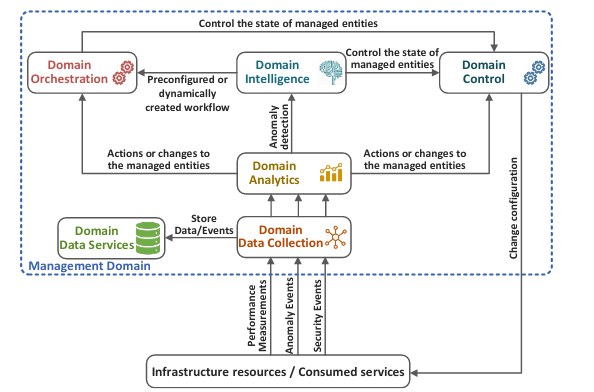
\includegraphics[width=\textwidth]{./fig/zsm-arch.png}
  \caption{معماری سطح بالای دامنه‌های مدیریتی \متن‌لاتین{ZSM}}
\end{figure}

\پاراگراف{}
هوش مصنوعی نقش قدرتمندی در کارکردهای خود مدیریتی ایفا می‌کند اما استفاده از هوش مصنوعی در \متن‌لاتین{ZSM} به وسیله حدود و ریسک‌های بسیاری محدود شده است.
از جمله‌ی این محدودیت‌ها می‌توان به محدودیت‌های قانونی، عملکرد کاملا خودکار سیستم و \نقاط‌خ اشاره کرد.


\قسمت{هوش تجربی شبکه}

\زیرقسمت{مقدمه}

\پاراگراف{}
کارگروه \متن‌لاتین{ETSI ENI} در حال طراحی یک معماری مدیریت شبکه شناختی\پانویس{Cognitive Network Management}
بر پایه حلقه بسته\پانویس{closed-loop} مکانیزم‌های هوش‌مصنوعی بر اساس سیاست‌های آگاه به متن\پانویس{Context-aware} و مبتنی بر داده‌ها
برای بهبود تجربه اپراتورهای شبکه می‌باشند.
این معماری بر پایه حلقه کنترلی، نظارت--ارزیابی--تصمیم--عمل می‌باشد.
این پروژه برای عملکردهای متنوع که مدیریت زیرساخت، عملیات‌های شبکه،
هماهنگی سرویس‌ها و تضمین آن‌ها را پوشش می‌دهند،‌ تعریف شده است.

\زیرقسمت{در قیاس با مدیریت شبکه و سرویس بدون لمس}

\پاراگراف{}
از بین کارکردهای \متن‌لاتین{ENI} آنچه به \متن‌لاتین{ZSM} مرتبط است
می‌توان به مدیریت هوشمند قطعه‌بندی شبکه، شناسایی و پیش‌بینی خطا در شبکه
و تظمین نیازمندی‌های سخت سرویس اشاره کرد.

\پاراگراف{}
برخلاف \متن‌لاتین{ZSM} که بر تکنیک‌های خودکارسازی، مدیریت انتها به انتها سرویس و
خودکارسازی کامل تمرکز دارد، \متن‌لاتین{ENI} بر تکنیک‌های هوش مصنوعی، مدیریت سیاست‌‌ها
و مکانیزم‌های حلقه بسته تمرکز دارد.

\قسمت{نتیجه‌گیری}

\پاراگراف{}
در این بخش معماری‌های \متن‌لاتین{NFV} و \متن‌لاتین{SFC} به صورت کامل شرح داده شد و اجزای آن‌ها و مسائل تحقیقاتی موجود در هر یک از این معماری‌ها بررسی شد.
همانگونه که بیان شد، معماری \متن‌لاتین{NFV} بر مجازی سازی کارکردها تمرکز دارد. یک سرویس در معماری \متن‌لاتین{NFV} با استفاده از \متن‌لاتین{NSD} توصیف می‌شود که شامل \متن‌لاتین{VNF}، \متن‌لاتین{VNF-FG}ها و لینک‌های توصیف کننده
ارتباطات بین \متن‌لاتین{VNF}ها است. معماری \متن‌لاتین{SFC} به ایجاد زنجیره پویا از کارکردها تمرکز دارد.

\پاراگراف{}
یک زنجیره کارکرد توسط یک گراف SFC توصیف می شود که به صورت مجموعه مرتب از کارکردها که ترافیک باید با ترتیب مشخصی از آن ها عبور کند توصیف می شود. این معماری تاکیدی بر مجازی سازی کارکردها ندارد. همچنین برای مسیریابی ترافیک در این معماری نیز می توان از سرآیند NSH استفاده کرد.همانگونه که بیان شد در حقیقت این دو معماری مکمل یکدیگر هستند و یک گراف SFC را می توان توسط یک VNF-FG معادل نمایش داد.
